\documentclass[conference]{IEEEtran}
\IEEEoverridecommandlockouts
% The preceding line is only needed to identify funding in the first footnote. If that is unneeded, please comment it out.
\usepackage{fontspec}
\setmainfont{TeX Gyre Termes}
\usepackage{cite}
\usepackage{amsmath,amssymb,amsfonts}
\usepackage{algorithmic}
\usepackage{graphicx}
\usepackage{textcomp}
\usepackage{xcolor}
\usepackage{listings}

\graphicspath{ {./figures/} }

\definecolor{codegreen}{rgb}{0,0.6,0}
\definecolor{codegray}{rgb}{0.5,0.5,0.5}
\definecolor{backcolour}{rgb}{0.6,0.6,0.6}

\lstset{
    commentstyle=\color{codegreen},
    keywordstyle=\color{blue},
    numberstyle=\tiny\color{codegray},
    stringstyle=\color{purple},
    basicstyle=\ttfamily\footnotesize,
    breaklines=true,                 
    captionpos=b,                    
    numbers=left,                    
    numbersep=5pt,                  
    showstringspaces=false,
    frame=single
}
\def\BibTeX{{\rm B\kern-.05em{\sc i\kern-.025em b}\kern-.08em
    T\kern-.1667em\lower.7ex\hbox{E}\kern-.125emX}}
\begin{document}

\title{Reprezentacje kodu źródłowego na potrzeby modeli i algorytmów głębokiego uczenia\\
% {\footnotesize \textsuperscript{*}Note: Sub-titles are not captured in Xplore and
% should not be used}
}

\author{\IEEEauthorblockN{1\textsuperscript{st} inż. Jędrzej Dubiak}
\IEEEauthorblockA{\textit{Wydział Elektryczny} \\
\textit{Politechnika Warszawska}\\
Warszawa, Polska \\
01178878@pw.edu.pl}
\and
\IEEEauthorblockN{2\textsuperscript{nd} inż. Rafał Pyłko}
\IEEEauthorblockA{\textit{Wydział Elektryczny} \\
\textit{Politechnika Warszawska}\\
Warszawa, Polska \\
01178878@pw.edu.pl}
\and
\IEEEauthorblockN{3\textsuperscript{rd} inż. Michał Jagodziński}
\IEEEauthorblockA{\textit{Wydział Elektryczny} \\
\textit{Politechnika Warszawska}\\
Warszawa, Polska \\
01178878@pw.edu.pl}
\and
\IEEEauthorblockN{4\textsuperscript{th} inż. Bartosz Dybowski}
\IEEEauthorblockA{\textit{Wydział Elektryczny} \\
\textit{Politechnika Warszawska}\\
Warszawa, Polska \\
01178878@pw.edu.pl}
\and
}

\maketitle

\renewcommand{\abstractname}{Streszczenie}
\begin{abstract}
TODO na koniec
\end{abstract}

\renewcommand{\IEEEkeywordsname}{Słowa kluczowe}
\begin{IEEEkeywords}
uczenie głębokie, reprezentacja kodu źródłowego
\end{IEEEkeywords}

\section{Wstęp}
Ostatnia dekada przyniosła ogromny postęp w dziedzinie uczenia maszynowego, szczególnie dzięki metodom uczenia głębokiego (Deep Learning), które zrewolucjonizowały obszary takie jak rozpoznawanie obrazów czy przetwarzanie języka naturalnego. Obecnie metody te są coraz szerzej adaptowane w inżynierii oprogramowania, gdzie wspomagają rozumienie i analizę programów komputerowych. Fundamentem sukcesu uczenia głębokiego w tym obszarze jest uczenie reprezentacji (representation learning), czyli proces przekształcania surowych danych w format, który modele mogą efektywnie przetwarzać \cite{b1}.

Reprezentacja kodu źródłowego to proces transformacji tekstowej postaci kodu programu w ustrukturyzowany, ogólny format wejściowy akceptowalny dla modeli uczenia głębokiego. Modele te nie są w stanie bezpośrednio zrozumieć surowego kodu źródłowego. Dlatego kod musi zostać przekształcony w taki sposób, aby skutecznie oddawał jego właściwości strukturalne, syntaktyczne oraz semantyczne \cite{b2}.

Głównym celem tworzenia reprezentacji kodu źródłowego jest umożliwienie modelom automatycznego wykrywania skomplikowanych wzorców w strukturach programów. Wybór konkretnej metody reprezentacji jest kluczowy, ponieważ determinuje on, jakie informacje o kodzie zostaną zachowane, a jakie utracone, co bezpośrednio wpływa na skuteczność algorytmu w danym zadaniu \cite{b3}.

\section{Taksonomia i formalne modelowanie reprezentacji kodu źródłowego}
W literaturze powtarza się dobrze utrwalona klasyfikacja reprezentacji kodu źródłowego ze względu na ich strukturę oraz poziom zawartej w nich informacji. Wyróżniamy reprezentacje leksykalne, syntaktyczne, semantyczne oraz hybrydowe i inne. 

Posłużmy się przykładem kodu źródłowego napisanego w języku C w celu rozróżnienia charakterystyki każdej z wymienionych reprezentacji.

\begin{lstlisting}[language=C, caption={Przykład kodu źródłowego do analizy reprezentacji \cite{b2}}]
void foo() {
  int x = source();
  if(x < MAX) {
    int y = 2*x;
    sink(y);
  }
}
\end{lstlisting}

\subsection{Reprezentacje Leksykalne (Token-based)}
Reprezentacja oparta na tokenach traktuje kod źródłowy jako wolny tekst lub płaską sekwencję znaków. Proces ten polega na konwersji kodu na listę tokenów, gdzie pojedynczym tokenem może być każde wyodrębnione słowo, a także każdy znak specjalny, taki jak nawias czy średnik.

Można wyróżnić kilka głównych podejść do podziału kodu na tokeny \cite{b1}:
\begin{itemize}
    \item Tokenizacja na poziomie słów - token reprezentuje wyrazy lub znaki specjalne.
    \item Tokenizacja na poziomie znaków - token reprezentuje pojedyńcze znaki.
    \item Tokenizacja na poziomie podsłów - kompromis między znakami, a słowami.
    \item Tokenizacja N-gram - token reprezentuje n-elementową sekwencję, np. pierwszy token to "void foo", a następny to "foo()", co dodaje informacje o kontekście sąsiadujących wyrazów.
\end{itemize}

\begin{lstlisting}[
    basicstyle=\ttfamily\small,
    breaklines=true,
    caption={Reprezentacja kodu w formie ztokenizowanej na poziomie słów \cite{b2}},
    frame=tb
]
['void', 'foo', '(', ')', '{', 'int', 'x', '=', 'source', '(', ')', ';', 
 'if', '(', 'x', '<', 'MAX', ')', '{', 'int', 'y', '=', '2*x', ';', 
 'sink', '(', 'y', ')', ';', '}', '}']
\end{lstlisting}

Aby modele Deep Learning mogły uczyć się z reprezentacji leksykalnej, tokeny są przekształcane na numeryczne wektory (embeddings) za pomocą statystycznych modeli językowych, takich jak word2vec lub doc2vec. Każdy token reprezentowany jest w ten sposób jako wektor liczb rzeczywistych \cite{b2}.

\subsection{Reprezentacje Syntaktyczne (Tree-based)}
Reprezentacja syntaktyczna modeluje kod poprzez uwzględnienie jego hierarchicznej struktury oraz reguł gramatyki użytego języka programowania. 

Najpopularniejszą strukturą w tym podejściu jest drzewo AST (Abstract Syntax Tree). Zamiast przetwarzać kod jako płaski ciąg znaków, AST konwertuje go w drzewo, w którym węzły reprezentują konkretne konstrukcje języka, takie jak wyrażenia, instrukcje, deklaracje \cite{b1}. Rysunek \ref{fig:tree_representation} przedstawia przykładową reprezentację kodu źródłowego w formie drzewa AST.

\begin{figure}[h]
    \centering
    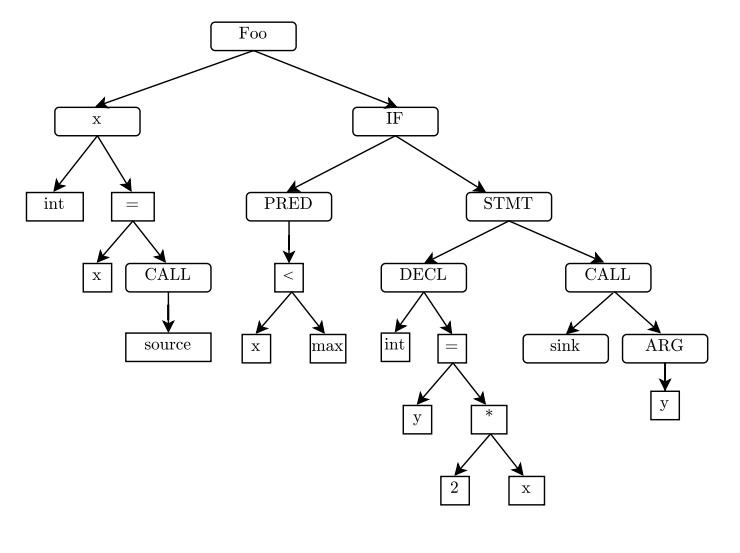
\includegraphics[width=\columnwidth]{tree-based.png}
    \caption{Reprezentacja kodu bazująca na strukturze drzewiastej \cite{b2}}
    \label{fig:tree_representation}
\end{figure}

\subsection{Reprezentacje Semantyczne (Graph-based)}

\begin{figure}[h]
    \centering
    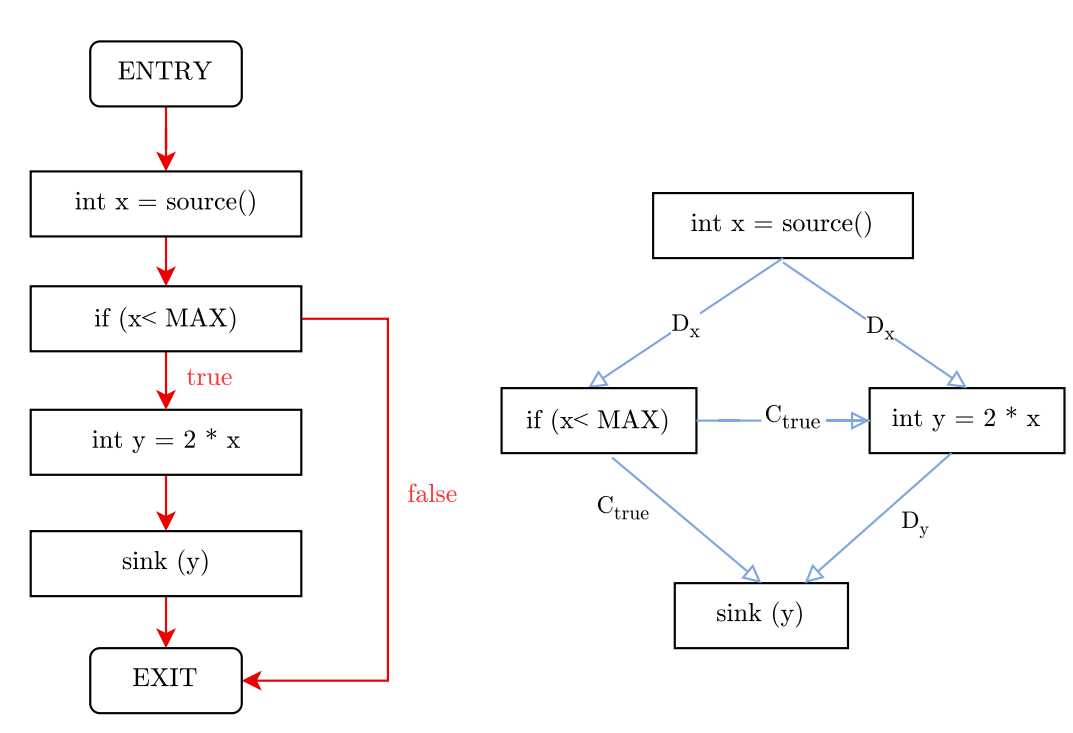
\includegraphics[width=\columnwidth]{graph-based.png}
    \caption{Reprezentacja kodu bazująca na grafach przepływu CFG i PDG \cite{b2}}
    \label{fig:graph_representation}
\end{figure}

\subsection{Reprezentacje Hybrydowe i Pośrednie}

\section{Zastosowanie reprezentacji kodu źródłowego w problemach inżynierii oprogramowania}
tutaj o taskach SE w jakich stosuje się reprezentację kodu źródłowego czyli wykrywanie podatności, podsumowywanie kodu, detekcja klonowania itp.

\section{Analiza skuteczności reprezentacji kodu źródłowego w problemach inżynierii oprogramowania}
Jakieś papiery z danymi o tym gdzie dana reprezentacja się najlepiej spisuje, ewentualnie zrobić swoją implementację i pokazać wyniki.

\section{Podsumowanie}
Wnioski dotyczące wyboru optymalnej reprezentacji w zależności od dostępnych zasobów i specyfiki problemu.

\renewcommand{\refname}{Bibliografia}
\begin{thebibliography}{00}
\bibitem{b1} Shanmugasundaram, D., Arivukkarasu, P., Chen, H., \& Cai, H. (2025). Deep Learning Representations of Programs: A Systematic Literature Review. ACM Computing Surveys, 58(5), 1-37.
\bibitem{b2} Samoaa, H. P., Bayram, F., Salza, P., \& Leitner, P. (2022). A systematic mapping study of source code representation for deep learning in software engineering. IET Software, 16(4), 351-385.
\bibitem{b3} Siow, J. K., Liu, S., Xie, X., Meng, G., \& Liu, Y. (2022, March). Learning program semantics with code representations: An empirical study. In 2022 IEEE international conference on software analysis, evolution and reengineering (SANER) (pp. 554-565). IEEE.
\bibitem{b4} Brauckmann, A., Goens, A., Ertel, S., \& Castrillon, J. (2020, February). Compiler-based graph representations for deep learning models of code. In Proceedings of the 29th International Conference on Compiler Construction (pp. 201-211).
\bibitem{b5} Casey, B., Santos, J. C., \& Perry, G. (2025). A survey of source code representations for machine learning-based cybersecurity tasks. ACM Computing Surveys, 57(8), 1-41.
\end{thebibliography}
\end{document}
